\section{Methodology}
\label{sec:methodology}

\subsection{CLEVR dataset}
The basis for my datasets is the Visual Question Answering (VQA) dataset CLEVR \citep{Johnson2017a}.
This dataset is split in two parts: a collection of images, and a set of questions and answers that refer and describe each image.
Many of the existing VQA datasets come with two problems.
First, they include many biases, such as biases in the base images and biases in the linguistic properties of the questions and answers.
A relatively high number of images of dogs in a dataset, might for instance bias a classifier model towards classifying dogs most of the time.
On the other hand, repeating patterns in the questions and answers might also be exploited by a model, without extracting the needed information from the image.
For these reasons the CLEVR dataset aims to reduce the biases as much as possible in both images and questions and answers.
Secondly, datasets may come with only a limited amount of annotations and information about the state in an image.
The CLEVR dataset uses artificially rendered 3D-scenes.
By doing so, all information about for instance the location of objects or their relations to each other can be saved and later used in training models or analyzing their results.

For this thesis, only the visual part of the dataset will be used and extended.
The questions and answers won't be used.
The visual part contains images of 3D-generated scenes depicting different kinds of simple objects.
Each of these objects is made up of a different combination of attributes, such as \emph{shape}, \emph{color}, \emph{size} and \emph{material}.
The possible values of these attributes are listed in Table \ref{tab:clevr-attributes}.
Three to ten objects are placed in random locations into the scene and assigned with random attributes.
To enhance realism and reduce ambiguity, objects are placed in a way that they do not intersect and have a certain distance from each other
Furthermore, it is made sure that every object is almost completely visible.
The position of the light and the camera are slightly jittered for each image to add noise reduce recurring patterns.
Figure \ref{fig:clevr-example} shows an example of a generated image in the CLEVR dataset.

\begin{table}[h]
    \centering
    \begin{tabular}{cccc}
        \toprule
        \textbf{ shape } & \textbf{ color } & \textbf{ size } & \textbf{ material } \\
        cube             & gray             & small           & rubber              \\
        sphere           & red              & large           & metal               \\
        cylinder         & blue                                                     \\
                         & green                                                    \\
                         & brown                                                    \\
                         & purple                                                   \\
                         & cyan                                                     \\
                         & yellow                                                   \\
        \bottomrule
    \end{tabular}
    \caption{Attributes of objects in the CLEVR dataset}
    \label{tab:clevr-attributes}
\end{table}

\begin{figure}[h]
    \centering
    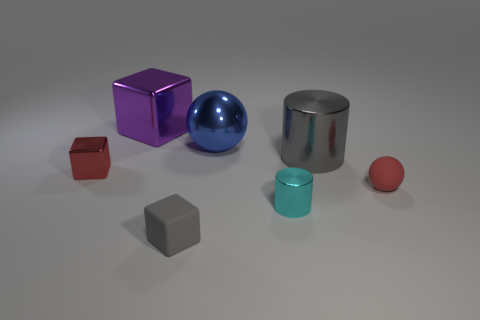
\includegraphics[width=.8\linewidth]{figures/CLEVR_example.png}
    \caption{Example of a generated image in the CLEVR dataset}
    \label{fig:clevr-example}
\end{figure}

Furthermore, the dataset contains information about each scene.
This includes all selected attributes for each object as well as the exact position of the centers of all the objects, both 3D-coordinates in the 3D scene and 2D-coordinates in the final rendered image.
In addition, simple spatial relations (in front of, behind, left, right) between the objects are calculated and stored.
These are simply based on the 3D-coordinates of the objects in relation to the position of the camera.

In this thesis, the code for the generation of the images is extended, and multiple new datasets are created.
The extension is detailed in section \ref{sec:creation-dataset}.


\subsection{Feature extractors}
In computer vision tasks, machines need to analyze images and extract information from them.
To do this, machines often rely on feature extractors.
Features are important parts or patterns in an image, which can have different levels of abstractions.
They can for example be low-level features, as geometric information about lines and edges in an image, or also very abstract information about whole objects.
Traditional approaches involve extracting key points and descriptors from an image and using them to represent the image \citep{Harris1988,Lowe1999,Bay2006}.
More recently, convolutional neural networks (CNN) became popular due to their ability to learn complex features automatically from raw image data.
These are also used in this thesis as a first layer to extract important information from the image. Hereby, two different architectures are tested.

First, I use the VGG19 \citep{Simonyan2015} which is an architecture based on many convolutional layers.
Using 16-19 convolutional layers with small convolution filters helps the model to solve localization and classification tasks on the training dataset, but also enables is to generalize onto other datasets.
After the convolutional layers, the data is passed first through an average pooling layer which outputs 512x7x7 dimensions.
Next follow three linear layers with \emph{ReLU} non-linearities in between.
After flattening the input, these classification layers output 4069, 4069 and 1000 dimensions respectively.

Secondly, I include the ResNet-101 \citep{He2016}.
This architecture tries to overcome the degradation of very deep networks, where the accuracy rapidly drops after it gets saturated.
This is done using residual blocks.
A residual block consists of two or three convolutional layers and a residual connection, also known as a shortcut connection.
The residual connection allows the input to be added directly to the output of the block, allowing the network to learn the residual function with respect to the input.
This approach enables the network to better preserve information from earlier layers and avoid the problem of information loss that can occur in very deep networks.
There are four blocks that output 256x56x56, 512x28x28, 1024x14x14 and 2048x1x1 dimensions.
A following average pooling layer outputs 2048x1x1 dimensions as well.
The final linear layer reduces the flattened data to 1000 dimensions, corresponding to the ImageNet classes.

Both architectures are available pretrained on an image classification task on the ImageNet dataset.
In this thesis, the implementations and weights available for PyTorch are used.\footnote{\href{https://pytorch.org/hub/pytorch\_vision\_resnet/}{https://pytorch.org/hub/pytorch\_vision\_resnet/}}\textsuperscript{,}\footnote{\href{https://pytorch.org/hub/pytorch\_vision\_vgg/}{https://pytorch.org/hub/pytorch\_vision\_vgg/}}
Since the task in this research is very different from a classification, it likely learned representations that are not directly transferrable to other tasks.
For this reason, multiple different adaptions of these architectures are compared.
Table \ref{tab:feature-extractor-archs} lists the different adaptions for both VGG19 and ResNet-101 that will be used in this research.
In the later chapters, it will be referred to these adaptions using the name in the table.

\begin{table}[h]
    \centering
    \begin{tabular}{rlc}
        \toprule
                            & \textbf{description}                                            & \textbf{ output dimensions } \\\midrule
        \textbf{VGG-0}      & contains only the convolutional layers                          & 512x7x7                      \\
        \textbf{VGG-avg}    & contains an additional average pooling layer                    & 512x7x7                      \\
        \textbf{VGG-cls1}   & \makecell[cl]{contains an additional one classification layer,                                 \\ including its non-linearity} & 4069                         \\
        \textbf{VGG-cls2}   & \makecell[cl]{contains another additional classification layer,                                \\ including its non-linearity} & 4069                         \\
        \textbf{VGG-cls3}   & the original VGG19 architecture                                 & 1000                         \\\midrule
        \textbf{ResNet-1}   & contains one residual block                                     & 256x56x56                    \\
        \textbf{ResNet-2}   & contains two residual blocks                                    & 512x28x28                    \\
        \textbf{ResNet-3}   & contains three residual blocks                                  & 1024x14x14                   \\
        \textbf{ResNet-4}   & contains four residual blocks                                   & 2048x1x1                     \\
        \textbf{ResNet-avg} & contains an additional average pooling layer                    & 2048x1x1                     \\
        \textbf{ResNet-cls} & the original ResNet-101 architecture                            & 1000                         \\
        \bottomrule
    \end{tabular}
    \caption{Different adaptions of VGG19 and ResNet-101 used in this research}
    \label{tab:feature-extractor-archs}
\end{table}

Furthermore, I experimented with both the pretrained models as well as with the architectures trained from scratch with a random initialization for the weights.
This reason for this was to test if the success of an experiment was actually making use of the pretrained knowledge incorporated in the models.
If that was not the case, the agents were likely not using image features, but instead relying on some other underlying patterns to solve the task.
Basically, this approach works as an indicator to determine the actual success of the agents aside from measures as the accuracy or precision.

\subsection{EGG framework}
The goal of this thesis is to run and compare different setups of language games systematically.
To do this, all experiments rely on the \emph{\textbf{E}mergence of lan\textbf{G}uage in \textbf{G}ames} (EGG) framework \citep{Kharitonov2019} which is implemented in PyTorch.
This framework consists of a heavily configurable core that controls the generating and parsing of the message, the calculation of the loss and the rules, for how the weights of all neural models are trained.
The configuration includes for example a choice between single symbol and sequence messages with varying RNNs, a choice between Gumbel-Softmax relaxation and REINFORCE algorithms to learn neural models containing discrete symbols or an easy switch between different loss functions.
Furthermore, runs of games can be saved to analyze the used messages of the agents and how they vary over the duration of the learning.

The framework is hereby setup in three levels.
Part of the lowest level are the \emph{agents} themselves.
The agents are neural models that need to be implemented from scratch and define how the agents process their input and in case of the receiver combine it with the message as well as what is their output.
The second level are \emph{wrappers} that take care of generating and parsing the message.
The sender wrapper uses the output of the sender agent, to produce a message.
The receiver on the other hand parses the message received by the sender and passes the result as an additional input to the receiver agent.
The third level, the \emph{game} links all described parts together.
It provides the agents with the input and passes the message from the sender to the receiver.
Furthermore, it uses the output of the receiver and calculates the loss, which is then the basis for the adaption of the weights for both wrappers and agents.

For the language games which are run in this thesis, the sender will always produce a sequence of symbols as a message, which the receiver will parse.
Gumbel-Softmax relaxation is applied to produce discrete symbols.
This is done using two LSTMs, an encoder LSTM in the sender wrapper and a decoder LSTM in the receiver wrapper.
The output of the sender agent is used as the initial hidden state for the encoder LSTM.
This LSTM is then producing symbols until it generates an end-of-sequence symbol.
This sequence is then passed to the receiver wrapper with its decoder LSTM.
Its hidden state is initialized randomly.
The received message sequence is processed symbol by symbol.
After each time, a symbol is processed by the LSTM, the resulting new hidden state is passed to the receiver agent as the parsed message.
The receiver agent is combining it with its representation of the image input and is predicting an output.
In other words the receiver agent produces as many outputs as symbols are present in the message.
The \emph{game} is then calculating a loss for each of these outputs separately.
These losses are summed up to a total loss that is used to adapt the weights in both agents as well as in both LSTMs.

\cmtDK{Gumbel-Softmax vs REINFORCE}

\subsection{Ethical considerations}
In the field of natural language processing (NLP) ethical issues often play major roles.
These can be part of the used datasets, the created models and their training as well as the application of the models.
For datasets, the role data privacy is increasing with the necessity of larger amounts of data \citep{Klymenko2022}.
Furthermore, datasets often contain biases, based for instance on the authors of the collected natural language texts. Often they also contain biases such as overrepresentations and underrepresentations.
Even though some of these biases are inherent to the data and not necessarily negative, much research is indicating that undetected and unaddressed biases in datasets might lead to negative consequences \citep{Shah2020,Field2021,Bender2021}.
Training neural models can also lead to environmental issues, as large models need to process huge amounts of data and require a lot of energy \citep{Bender2021}.
Finally, the application of trained models can create harm.
This applies for example to easy accessible large language model (LLMs) that can be used to create information hazard \citep{Weidinger2022}.

The research in this thesis tries to reduce these risks.
Looking at the datasets that are used in this thesis, all data is created artificially and contains therefore no personal information.
Even further, the aim of the creation of these datasets is to reduce biases.
It doesn't include any social information, but on the other hand consists only of abstract scenes.
The choice of which attributes the objects are made up is inherently biased towards human cognition, but doesn't have a social impact.
The models and agents are therefore trained, by including as few human biases as possible.

Looking at the environmental issues, the models used in this thesis consist of only few trained layers and the training is therefore short and doesn't require much energy.
Larger models as the feature extractors are already pretrained and add no additional consumption.

Finally, the purpose of this thesis is to analyze the results and the emerged language and draw conclusions, how emerged languages can be grounded better in the environment.
For that reason, the final models can't be uses in any real world applications and produce potential harm.
